\documentclass{article}
\usepackage[T1]{fontenc}
\usepackage{lmodern}
\usepackage{graphicx}
\usepackage{amsmath,amssymb}
\usepackage[a4paper,margin=2cm]{geometry}
\usepackage[absolute,overlay]{textpos}
\setlength{\TPHorizModule}{1mm}
\setlength{\TPVertModule}{1mm}
\usepackage[indonesian]{babel}
\usepackage{hyperref}
\setlength{\emergencystretch}{2em}
% unit: Halaman 84

\begin{document}

% === Halaman 84 (python/native) ===

84

• Dengan 

menggunakan 

tabel 

frekuensi 

kemunculan pasangan huruf di dalam Bahasa 

Inggris dan cipherteks yang cukup banyak, 

Playfair cipher dapat dipecahkan.

• Kelemahan lainnya, bigram dan kebalikannya 

(misal AB dan BA) akan didekripsi menjadi pola 

huruf plainteks yang sama (misal RE dan ER). Di 

dalam bahasa Inggris terdapat banyak kata yang 

mengandung bigram terbalik seperti REceivER 

dan DEpartED.

% deskripsi: gambar native xref 301
\noindent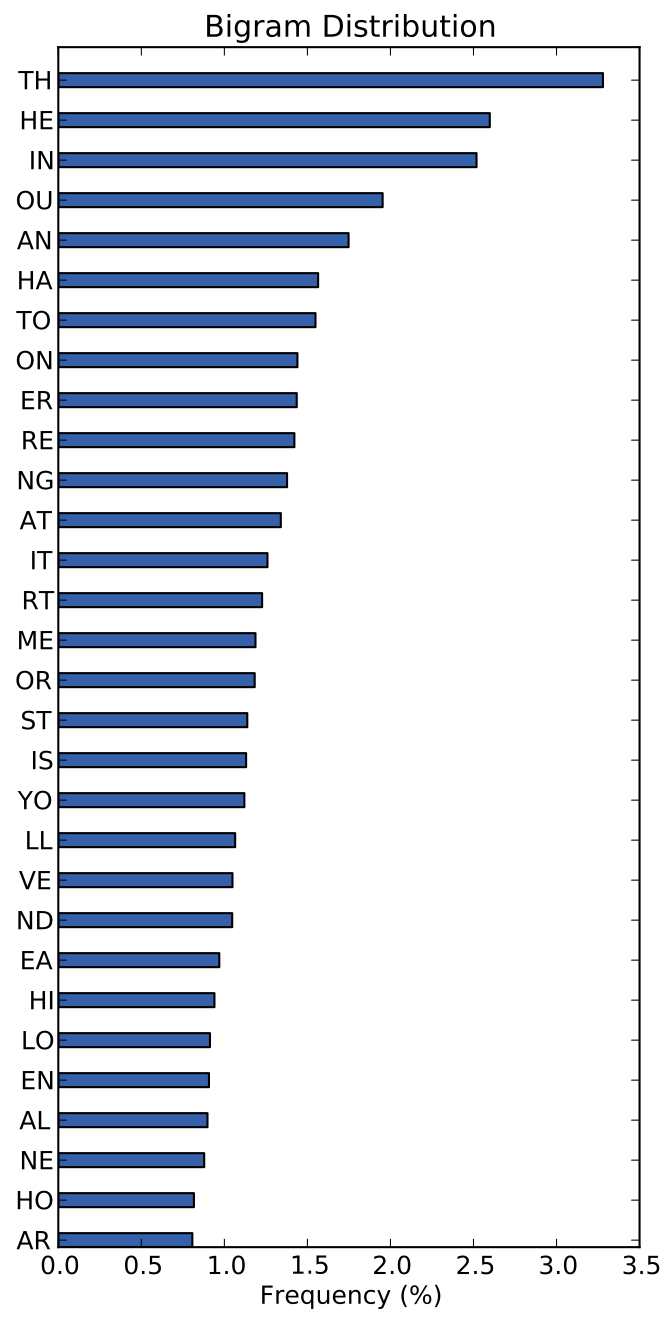
\includegraphics[width=0.85\textwidth]{../../images/python/page_084_img_01.png}

\end{document}
